\documentclass{article}
\usepackage{graphicx}
\usepackage{multirow}
\usepackage[utf8]{inputenc}
\usepackage{listings}
\usepackage{xcolor}
\usepackage{rotating}

\definecolor{codegreen}{rgb}{0,0.6,0}
\definecolor{codegray}{rgb}{0.5,0.5,0.5}
\definecolor{codepurple}{rgb}{0.58,0,0.82}
\definecolor{backcolour}{rgb}{0.95,0.95,0.92}

\lstdefinestyle{mystyle}{
	backgroundcolor=\color{backcolour},   
	commentstyle=\color{codegreen},
	keywordstyle=\color{magenta},
	numberstyle=\tiny\color{codegray},
	stringstyle=\color{codepurple},
	basicstyle=\ttfamily\footnotesize,
	breakatwhitespace=false,         
	breaklines=true,                 
	captionpos=b,                    
	keepspaces=true,                 
	numbers=left,                    
	numbersep=5pt,                  
	showspaces=false,                
	showstringspaces=false,
	showtabs=false,                  
	tabsize=2
}

\lstset{style=mystyle}

\usepackage[a4paper, total={6in, 8in}]{geometry}
\title{Assignment 1 \\
		Analysis and Report}
\author{Student ID : 28993373\\
	Bhanuka Manesha Samarasekara Vitharana Gamage\\
	bsam0002@student.monash.edu\\
	School of Information Technology}

\begin{document}
	\lstset{language=Python}   
	\maketitle
	
	\section{Proof of the Heuristic Function}
	
	The \emph{input1.txt} example is shown below :
	
	\begin{figure}[!h]
		\centering
		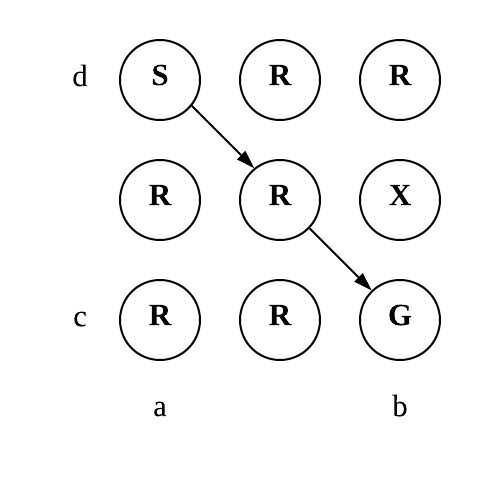
\includegraphics[width=50mm]{img1.png}
		\caption{Minimum Heuristic from Start to Goal for \emph{input1.txt}}
		\label{fig:img1}
	\end{figure}
	
	Using the above example, we will prove that the heuristic is valid. The heuristic used in this case is the maximum between the difference from the current state to the goal state. The derivation of $h(n)$ is stated below:
	
	\begin{equation} 
		dx = | b - a | \label{equation:2}
	\end{equation}
	\begin{equation} 
		dy = | d - c | \label{equation:3}
	\end{equation}
	
	\begin{equation}
		h(n) = max(dx,dy) \label{equation:4}
	\end{equation}
	
	Below is the python implementation for the heuristic:

		\newpage
		\begin{lstlisting}[language=Python]
		def heuristic(self,x,y):
			'''
			method used to calculate the heuristic value given the 
			current x and y coordinates
			@param x: current x coordinate
			@param y: current y coordinate
			@return: returns the heuristic value
			'''
			# Calculate the difference in both x and y directions
			dx = abs(x - self.GOAL_COORD[0])
			dy = abs(y - self.GOAL_COORD[1])
			
			# Returns the max of either the x or y direction
			return max(dx,dy)
		\end{lstlisting}

	 When determining the heuristic we assume that there are no ridges in the map. Therefore the rules are relaxed compared to the actual rules of the environment. 
	In order for the heuristic to be valid, it needs to be admissible and monotonic. Now let us prove that the above heuristic is Admissible and Monotonic.
	
	\subsection{Admissibility}
	
		In order for a heuristic to be admissible it needs to satisfy :
		\begin{equation}
			\forall n \quad h(n) \le h*(n) \label{equation:1}
		\end{equation}
		
		Using Figure \ref{fig:img1} we can derive the following equations:
		
		Since we get the maximum value between dx and dy as the heuristic, it will always be the minimum amount of diagonal moves between the start and goal state. Therefore we can deduce that any cost will be greater than the heuristic and will never be less than it. So for the best case the heuristic will be equal to the actual cost, but for the worst case the heuristic will be underestimating since the cost of non-diagonal moves are greater than one.
		
		Therefore the above heuristic is admissible as it satisfy Equation \ref{equation:1} and it does not overestimate the cost.
		
	\subsection{Monotonicity}
		In order for a heuristic to be monotonic, it should satisfy the following condition:
		\begin{equation}
			\forall n \quad h(n) \le c(m,n) + h(m) \label{equation:5}
		\end{equation}
		\begin{center}
			where m is a child of n
		\end{center}
	
		Using the same example from above (Figure \ref{fig:img1}), we can prove that the heuristic of any given node is less than or equal to the cost from that node to its successor plus the heuristic of the successor. This is because we take the max difference between the current node and the goal node.
	
		\subsection{Is the resulting algorithm A or A*?}
		Therefore since the actual cost is always used for the $g(n)$ value and not an estimate, we can state that the resulting algorithm is A*. 
		\newpage
	\section{Tie Breaker Implementation}
	
	As show below, to implement the tie breaker, we override the Node instance's less than operator:
			\begin{lstlisting}[language=Python]
    def __lt__(self, other):
			'''
			This method is used to override the less than operator in
			python to use the f cost for comparison
			@param other: the other node to be compared
			@return: boolean value stating whether its less than or not
			'''
			if (self.f < other.f):
				return True
			elif(self.f == other.f ):
				if self.operator in self.best_operators:
					return True
				elif other.operator in other.best_operators:
					return False
				else:
					return True
			else:
				return False
	\end{lstlisting}
	
	As per line 10, if the cost of the nodes are equal, we prioritize the node which was generated using a diagonal operator such as ``LU, LD, RU, RD''. So the tie breaker implementation will always prioritize paths with diagonals.
	
	\section{Test Cases}
	\subsection{Output for all the test cases}
		Below are the test cases and the resulting path from each algorithm:
		
		\subsubsection{input1.txt}
			\begin{lstlisting}
				3
				SRR
				RRX
				RRG
					
				DLS : S-RD-D-R-G 5
				A* : S-RD-D-R-G 5
		\end{lstlisting}
	
	\subsubsection{input2.txt}
		\begin{lstlisting}
				5
				SRRXG
				RXRXR
				RRRXR
				XRXRR
				RRRRX
				
				DLS : S-D-D-R-D-D-R-R-U-R-U-U-U-G 24
				A* : S-D-D-R-D-D-R-R-U-R-U-U-U-G 24
		\end{lstlisting}
	
	\subsubsection{input3.txt}
		\begin{lstlisting}
				5
				SRXXX
				RRRXG
				XRRRR
				XRRRR
				RXXRX
		
				DLS : S-RD-RD-RD-RU-U-G 6
				A* :  S-RD-RD-RD-RU-U-G 6
		\end{lstlisting}
	
	\subsubsection{input4.txt}
		\begin{lstlisting}
				7
				RRRXRRR
				RXRRRXR
				RXXXXXR
				RRXSXXR
				XRXRXXR
				XRXRXXR
				XRRRXGR
				
				DLS : S-D-D-D-L-L-U-U-U-L-U-U-U-R-R-D-R-R-U-R-R-D-D-D-D-D-D-L-G 54
				A* : S-D-D-D-L-L-U-U-U-L-U-U-U-R-R-D-R-R-U-R-R-D-D-D-D-D-D-L-G 54
		\end{lstlisting}
	
	\subsubsection{input5.txt}
		\begin{lstlisting}
				5
				SRRRG
				RRRRR
				XXXXX
				RRRRR
				RRRRR
				
				DLS : S-RD-R-R-RU-G 6
				A* : S-RD-RU-RD-RU-G 4
		\end{lstlisting}
	
	\subsubsection{input6.txt}
		\begin{lstlisting}
				100
				Too big to display here...
				
				DLS : S-RD-R-D-D-D-R-R-RD-RU-R-R-RD-RD-RD-RU-U-U-U-U-R-R-R-R-RD-RD-RD-RD-RD-RU-U-U-U-U-R-R-R-R-RD-RD-RD-RD-RD-RU-U-U-U-U-R-R-R-R-RD-RD-RD-RD-RD-RU-U-U-U-U-R-R-R-R-RD-RD-RD-RD-RD-RU-U-U-U-U-R-R-R-R-RD-RD-RD-RD-RD-RU-U-U-U-U-R-R-R-R-RD-RD-RD-RD-RD-RU-U-U-U-U-R-R-R-R-RD-RD-RD-RD-RD-RU-U-U-U-U-R-R-R-R-RD-RD-RD-RD-RD-RU-U-U-U-U-R-R-R-R-RD-RD-RD-D-D-D-D-G 226
				A* : S-RD-RU-R-R-RU-RD-R-R-U-RU-RD-RD-RD-D-R-R-R-R-RU-RD-RD-RD-RU-RU-R-R-R-R-RU-RD-RD-RD-RU-RU-R-R-R-R-RU-RD-RD-RD-RU-RU-R-R-R-R-RU-RD-RD-RD-RU-RU-R-R-R-R-RU-RD-RD-RD-RU-RU-R-R-R-R-RU-RD-RD-RD-RU-RU-R-R-R-R-RU-RD-RD-RD-RU-RU-R-R-R-R-RU-RD-RD-RD-RU-RU-R-R-R-R-RD-LD-RD-RD-RD-LD-RD-G 147
		\end{lstlisting}
	\newpage
		\subsubsection{input7.txt}
	\begin{lstlisting}
			4
			XRGR
			SXRR
			RRXR
			RRRX
			
			
			DLS : NO-PATH
			A* : NO-PATH
	\end{lstlisting}
	
		\subsubsection{input8.txt}
	\begin{lstlisting}
			6
			SRRRRR
			RRRXXR
			RXRRRR
			RRXRXR
			XRRRRR
			GRRRXR
			
			DLS : S-RD-R-D-R-D-D-LD-L-L-G 16
			A* : S-D-D-D-R-D-D-L-G 14
	\end{lstlisting}
	
		\subsubsection{input9.txt}
	\begin{lstlisting}
			6
			RSRXGR
			RXRXRR
			RRXRXR
			RRRRXR
			RXRXRR
			RRRRRR
			
			DLS : S-L-D-D-RD-R-D-D-R-R-RU-U-U-U-LU-G 25
			A* : S-L-D-D-RD-R-D-D-R-R-RU-U-U-U-LU-G 25
	\end{lstlisting}
	
	
	
	\section{Analysis}
	In order to perform an analysis, multiple test cases were generated and tested on the two algorithms. Below is a table with the time taken for each input by the two algorithms. Please do note that each time is an average of five run.

	\newpage
	\begin{sidewaystable}[!h]
		\begin{tabular}{|c|c|l|l|l|l|l|l|l|l|l|l|l|}
			\hline
			\multirow{3}{*}{\textbf{Input File}} & \multicolumn{12}{c|}{\textbf{Time Taken}}                                                                   \\ \cline{2-13} 
			& \multicolumn{6}{c|}{\textbf{DLS}}                                        & \multicolumn{6}{c|}{\textbf{A*}} \\ \cline{2-13} 
			& \multicolumn{1}{l|}{1} & 2                         & 3 & 4 & 5 & \textbf{Average} & 1  & 2  & 3  & 4  & 5  & \textbf{Average}  \\ \hline
			input1.txt                           &0.00024 &	0.00017&	0.00023&	0.00017&	0.00017&	\textbf{0.00020}	&0.00028&	0.00028&	0.00028	&0.00033&	0.00028&	\textbf{0.00029 }   \\ \hline
			
			input2.txt                           & 0.00068	& 0.00048	&0.00047&	0.00048&	0.00049	&\textbf{0.00052}&	0.00067&	0.00067&	0.00065	&0.00067&	0.00067&\textbf{	0.00067  }   \\ \hline
			
			input3.txt                           & 0.00035&	0.00034&	0.00035	&0.00035&	0.00035	&\textbf{0.00035}	&0.00081&	0.00068	&0.00058&	0.00057	&0.00057&	\textbf{0.00064     }\\ \hline
			
			input4.txt                           & 0.00073 &	0.00073&	0.00072	&0.00072&	0.00084&	\textbf{0.00075}	&0.00152&	0.00152&	0.00150&	0.00152&	0.00150&\textbf{	0.00151 }   \\ \hline
			
			input5.txt                           & 0.00035 &	0.00027	& 0.00027	&0.00027	& 0.00027	&\textbf{0.00029}	&0.00029	&0.00029	&0.00028	&0.00027& 	0.00029	&\textbf{0.00028 }   \\ \hline
			
			input6.txt                           & 0.08533	&0.08353&	0.08298&	0.08362	&0.08385&	\textbf{0.08386}&	10.35549&	11.44547&	10.61212&	11.73250&	11.42238& 	\textbf{11.11359   }\\ \hline
			
			input7.txt                           & 0.00026	& 0.00021& 	0.00023& 	0.00022	& 0.00022& 	\textbf{0.00023}& 	0.00022& 	0.00026& 	0.00023	& 0.00023	& 0.00023	& \textbf{0.00023   } \\ \hline
			
			input8.txt                           & 0.00061	&0.00059&	0.00049&	0.00049	&0.00050&\textbf{0.00054}	&0.00081&	0.00082	&0.00087&	0.00083	&0.00083&	\textbf{0.00083 }   \\ \hline
			
			input9.txt                           & 0.00090	&0.00089&	0.00089&	0.00087&	0.00088&	\textbf{0.00089}&	0.00102	&0.00103&	0.00102	&0.00104&	0.00103&	\textbf{0.00103 }   \\ \hline
		\end{tabular}
	\caption{Time Taken for each Algorithm on each input file}
	\end{sidewaystable}
	

	
\end{document}